% !TEX root = ../../../main.tex
% 来源：中学数学实验教材·第一册（代数）
% 章节：有理数系 / 有理数的意义
% 原始文件：1.tex，行 1315-1330
% 类型：tikz
% ---
		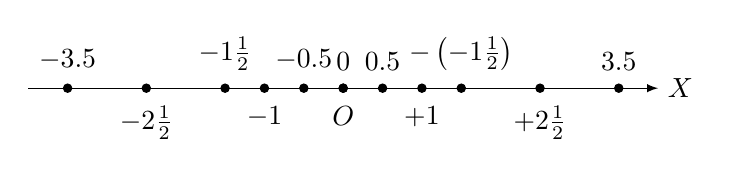
\begin{tikzpicture}[>=latex]
		\draw [fill=black] (0,0) circle(1.5pt) node[below=3pt]{$O$};
		\draw [fill=black] (0,0) circle(1.5pt) node[above=3pt]{$0$};
		\draw [fill=black] (1,0) circle(1.5pt) node[below=3pt]{$+1$};
		\draw [fill=black] (-1,0) circle(1.5pt)node[below=3pt]{$-1$};
		\draw [fill=black] (-.5,0) circle(1.5pt)node[above=3pt]{$-0.5$};
		\draw [fill=black] (.5,0) circle(1.5pt)node[above=3pt]{$0.5$};
		\draw [fill=black] (1.5,0) circle(1.5pt)node[above=3pt]{$-\left(-1\frac{1}{2}\right)$};
		\draw [fill=black] (-1.5,0) circle(1.5pt)node[above=3pt]{$-1\frac{1}{2}$};
		\draw [fill=black] (-3.5,0) circle(1.5pt)node[above=3pt]{$-3.5$};
		\draw [fill=black] (3.5,0) circle(1.5pt)node[above=3pt]{$3.5$};
		\draw [fill=black] (2.5,0) circle(1.5pt) node[below=3pt]{$+2\frac{1}{2}$};
		\draw [fill=black] (-2.5,0) circle(1.5pt)node[below=3pt]{$-2\frac{1}{2}$};
		\draw[->] (-4,0)--(4,0)node [right]{$X$};
		
		\end{tikzpicture}
